%!TEX root = forallxsol.tex
%\part{Interpretations}
%\label{ch.semantics}
%\addtocontents{toc}{\protect\mbox{}\protect\hrulefill\par}

\stepcounter{chapter} % Extensionality

\chapter{Truth in FOL}\setcounter{ProbPart}{0}
\problempart
\label{pr.TorF1}
Consider the following interpretation:
	\begin{ebullet}
		\item The domain comprises only Corwin and Benedict
		\item `$\atom{A}{x}$' is to be true of both Corwin and Benedict
		\item `$\atom{B}{x}$' is to be true of Benedict only
		\item `$\atom{N}{x}$' is to be true of no one
		\item `$c$' is to refer to Corwin
	\end{ebullet}
Determine whether each of the following sentences is true or false in that interpretation:
\begin{earg}
\item $\atom{B}{c}$ \hfill \myanswer{False}
\item $\atom{A}{c} \eiff \enot \atom{N}{c}$ \hfill \myanswer{True}
\item $\atom{N}{c} \eif (\atom{A}{c} \eor \atom{B}{c})$ \hfill \myanswer{True}
\item $\forall x\,\atom{A}{x}$ \hfill \myanswer{True}
\item $\forall x \enot \atom{B}{x}$ \hfill \myanswer{False}
\item $\exists x(\atom{A}{x} \eand \atom{B}{x})$ \hfill \myanswer{True}
\item $\exists x(\atom{A}{x} \eif \atom{N}{x})$ \hfill \myanswer{False}
\item $\forall x(\atom{N}{x} \eor \enot \atom{N}{x})$ \hfill \myanswer{True}
\item $\exists x\,\atom{B}{x} \eif \forall x\,\atom{A}{x}$ \hfill \myanswer{True}
\end{earg}

\problempart
\label{pr.TorF2}
Consider the following interpretation:	
	\begin{ebullet}
		\item The domain comprises only Lemmy, Courtney and Eddy
		\item `$\atom{G}{x}$' is to be true of Lemmy, Courtney and Eddy.
		\item `$\atom{H}{x}$' is to be true of and only of Courtney
		\item `$\atom{M}{x}$' is to be true of and only of Lemmy and Eddy
		\item `$c$' is to refer to Courtney
		\item `$e$' is to refer to Eddy
	\end{ebullet}
Determine whether each of the following sentences is true or false in that interpretation:
\begin{earg}
\item $\atom{H}{c}$ \hfill \myanswer{True}
\item $\atom{H}{e}$\hfill \myanswer{False}
\item $\atom{M}{c} \eor \atom{M}{e}$ \hfill \myanswer{True}
\item $\atom{G}{c} \eor \enot \atom{G}{c}$ \hfill \myanswer{True}
\item $\atom{M}{c} \eif \atom{G}{c}$ \hfill \myanswer{True}
\item $\exists x\,\atom{H}{x}$ \hfill \myanswer{True}
\item $\forall x\,\atom{H}{x}$ \hfill \myanswer{False}
\item $\exists x \enot \atom{M}{x}$ \hfill \myanswer{True}
\item $\exists x(\atom{H}{x} \eand \atom{G}{x})$ \hfill \myanswer{True}
\item $\exists x(\atom{M}{x} \eand \atom{G}{x})$ \hfill \myanswer{True}
\item $\forall x(\atom{H}{x} \eor \atom{M}{x})$ \hfill \myanswer{True}
\item $\exists x\,\atom{H}{x} \eand \exists x\,\atom{M}{x}$ \hfill \myanswer{True}
\item $\forall x(\atom{H}{x} \eiff \enot \atom{M}{x})$ \hfill \myanswer{True}
\item $\exists x\,\atom{G}{x} \eand \exists x \enot \atom{G}{x}$ \hfill \myanswer{False}
\item $\forall x\exists y(\atom{G}{x} \eand \atom{H}{y})$ \hfill \myanswer{True}
\end{earg}

\problempart
\label{pr.TorF3}
Following the diagram conventions introduced at the end of \S23, consider the following interpretation:	
\begin{center}
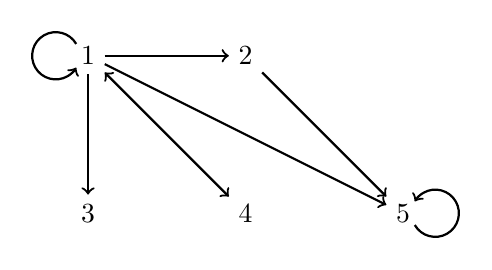
\begin{tikzpicture}
\node (atom1) at (0,2) {1};
\node (atom2) at (2,2) {2};
\node (atom4) at (0,0) {3};
\node (atom5) at (2,0) {4};
\node (atom6) at (4,0) {5};
\draw[->, thick] (atom1)+(-0.15,0.15) arc (-330:-30:.3); 
\draw[->, thick] (atom6)+(0.15,-0.15) arc (-150:150:.3); 
\draw[->, thick] (atom1) -- (atom2);
\draw[->, thick] (atom1) -- (atom4);
\draw[<->, thick] (atom1) -- (atom5);
\draw[->, thick] (atom1) -- (atom6);
\draw[->, thick] (atom2) -- (atom6);
\end{tikzpicture}
\end{center}
Determine whether each of the following sentences is true or false in that interpretation:
\begin{earg}
\item $\exists x\,\atom{R}{x,x}$ \hfill \myanswer{True}
\item $\forall x\,\atom{R}{x,x}$ \hfill \myanswer{False}
\item $\exists x \forall y\,\atom{R}{x,y}$ \hfill \myanswer{True}
\item $\exists x \forall y\,\atom{R}{y,x}$ \hfill \myanswer{False}
\item $\forall x \forall y \forall z ((\atom{R}{x,y} \eand \atom{R}{y,z}) \eif \atom{R}{x,z})$ \hfill \myanswer{False}
\item $\forall x \forall y \forall z ((\atom{R}{x,y} \eand \atom{R}{x,z}) \eif \atom{R}{y,z})$ \hfill \myanswer{False}
\item $\exists x \forall y \enot \atom{R}{x,y}$ \hfill \myanswer{True}
\item $\forall x(\exists y\,\atom{R}{x,y} \eif \exists y\,\atom{R}{y,x})$ \hfill \myanswer{True}
\item $\exists x \exists y (\enot x = y \eand \atom{R}{x,y} \eand \atom{R}{y,x})$ \hfill \myanswer{True}
\item $\exists x \forall y(\atom{R}{x,y} \eiff x = y)$ \hfill \myanswer{True}
\item $\exists x \forall y(\atom{R}{y,x} \eiff x = y)$ \hfill \myanswer{False}
\item $\exists x \exists y(\enot x = y \eand \atom{R}{x,y} \eand \forall z(\atom{R}{z,x} \eiff y = z))$ \hfill \myanswer{True}
\end{earg}

\stepcounter{chapter} % Semantic concepts

\chapter{Using Interpretations}\setcounter{ProbPart}{0}

\solutions
\problempart
\label{pr.Contingent}
Show that each of the following is neither a validity nor a contradiction:
\begin{earg}
\item \leftsolutions\ $\atom{D}{a} \eand \atom{D}{b}$
\item \leftsolutions\ $\exists x\,\atom{T}{x,h}$
\item \leftsolutions\ $\atom{P}{m} \eand \enot\forall x\,\atom{P}{x}$
\item $\forall z\, \atom{J}{z} \eiff \exists y\,\atom{J}{y}$
\item $\forall x (\atom{W}{x,m,n} \eor \exists y\atom{L}{x,y})$
\item $\exists x (\atom{G}{x} \eif \forall y\,\atom{M}{y})$
\item $\exists x (x = h \eand x = i)$
\end{earg}

\solutions
\problempart
\label{pr.NotEquiv}
Show that the following pairs of sentences are not logically equivalent.
\begin{earg}
\item $\atom{J}{a}$, $\atom{K}{a}$
\item $\exists x\,\atom{J}{x}$, $\atom{J}{m}$
\item $\forall x\,\atom{R}{x,x}$, $\exists x\,\atom{R}{x,x}$
\item $\exists x\,\atom{P}{x} \eif \atom{Q}{c}$, $\exists x (\atom{P}{x} \eif \atom{Q}{c})$
\item $\forall x(\atom{P}{x} \eif \enot \atom{Q}{x})$, $\exists x(\atom{P}{x} \eand \enot \atom{Q}{x})$
\item $\exists x(\atom{P}{x} \eand \atom{Q}{x})$, $\exists x(\atom{P}{x} \eif \atom{Q}{x})$
\item $\forall x(\atom{P}{x}\eif \atom{Q}{x})$, $\forall x(\atom{P}{x} \eand \atom{Q}{x})$
\item $\forall x\exists y\,\atom{R}{x,y}$, $\exists x\forall y\,\atom{R}{x,y}$
\item $\forall x\exists y\,\atom{R}{x,y}$, $\forall x\exists y\,\atom{R}{y,x}$
\end{earg}


\problempart
Show that the following sentences are jointly satisfiable:
\begin{earg}
\item $\atom{M}{a}, \enot \atom{N}{a}, Pa, \enot \atom{Q}{a}$
\item $\atom{L}{e,e}, \atom{L}{e,g}, \enot \atom{L}{g,e}, \enot \atom{L}{g,g}$
\item $\enot (\atom{M}{a} \eand \exists x\,\atom{A}{x}), Ma \eor \atom{F}{a}, \forall x(\atom{F}{x} \eif \atom{A}{x})$
\item $\atom{M}{a} \eor \atom{M}{b}, \atom{M}{a} \eif \forall x \enot \atom{M}{x}$
\item $\forall y\,\atom{G}{y}, \forall x (\atom{G}{x} \eif \atom{H}{x}), \exists y \enot \atom{I}{y}$
\item $\exists x(\atom{B}{x} \eor \atom{A}{x}), \forall x \enot \atom{C}{x}, \forall x\bigl[(\atom{A}{x} \eand \atom{B}{x}) \eif Cx\bigr]$
\item $\exists x\,\atom{X}{x}, \exists x\,\atom{Y}{x}, \forall x(\atom{X}{x} \eiff \enot \atom{Y}{x})$
\item $\forall x(\atom{P}{x} \eor \atom{Q}{x}), \exists x\enot(\atom{Q}{x} \eand \atom{P}{x})$
\item $\exists z(\atom{N}{z} \eand \atom{O}{z,z}), \forall x\forall y(\atom{O}{x,y} \eif \atom{O}{y,x})$
\item $\enot \exists x \forall y\,\atom{R}{x,y}, \forall x \exists y\,\atom{R}{x,y}$
\item $\enot \atom{R}{a,a}$, $\forall x (x=a \eor \atom{R}{x,a})$
\item $\forall x\forall y\forall z[(x=y \eor y=z )\eor x=z]$, $\exists x\exists y\ \enot x= y$
\item $\exists x\exists y((\atom{Z}{x} \eand \atom{Z}{y} )\eand x=y)$, $\enot \atom{Z}{d}$, $d=e$
\end{earg}

\problempart
Show that the following arguments are invalid:
\begin{earg}
\item $\forall x(\atom{A}{x} \eif \atom{B}{x}) \therefore \exists x\,\atom{B}{x}$
\item $\forall x(\atom{R}{x} \eif \atom{D}{x}), \forall x(\atom{R}{x} \eif \atom{F}{x}) \therefore \exists x(\atom{D}{x} \eand \atom{F}{x})$
\item $\exists x(\atom{P}{x}\eif \atom{Q}{x}) \therefore \exists x\,\atom{P}{x}$
\item $\atom{N}{a} \eand \atom{N}{b} \eand \atom{N}{c} \therefore \forall x\,\atom{N}{x}$
\item $\atom{R}{d,e}, \exists x\,\atom{R}{xd} \therefore \atom{R}{e,d}$
\item $\exists x(\atom{E}{x} \eand \atom{F}{x}), \exists x\,\atom{F}{x} \eif \exists x\,\atom{G}{x} \therefore \exists x(\atom{E}{x} \eand \atom{G}{x})$
\item $\forall x\,\atom{O}{x,c}, \forall x\,\atom{O}{c,x} \therefore \forall x\,\atom{O}{x,x}$
\item $\exists x(\atom{J}{x} \eand \atom{K}{x}), \exists x \enot \atom{K}{x}, \exists x \enot \atom{J}{x} \therefore \exists x(\enot \atom{J}{x} \eand \enot \atom{K}{x})$
\item $\atom{L}{a,b} \eif \forall x\,\atom{L}{x,b}, \exists x\,\atom{L}{x,b} \therefore \atom{L}{b,b}$
\item $\forall x(\atom{D}{x} \eif \exists y\,\atom{T}{y,x}) \therefore \exists y \exists z\ \enot y= z$
\end{earg}

\stepcounter{chapter} % Reasoning about interpretations